



%----------------------------------------------------------------------------------------

\newpage

% Section : Reproducibility


\section{Reproducibility}{Reproducibilité}



%----------------------------------------------------------------------------------------



\comment{(JR) évoquer l'accessibilité des bases de données, le manque de Data papers, la fermeture et méfiance, le travail supplémentaire à recoder. Evoquer Energy Price (reviewers bronchent pas ! ).}


\comment[JR]{evoquer ouverture des cours, formation interdisciplinaire etc. : pas ici, plutot en ouverture finale ?}


\comment[JR]{expérience de reviewer sur reproductibilité directe des papiers soumis. ex. plosOne se réfugient derrière ``synthetic data are not data''}



The strength of science comes from the cumulative and collective nature of research \comment{(Florent) pas besoin de repartir d'aussi loin}
, as progresses are made as Newton said ``standing on the shoulder of giants'', meaning that the scientific enterprise at a given time relies on all the work done before and that advances would not be possible without constructing on it. It includes development of new theories, but also extension, testing or falsifiability of previous ones. In that context 




\bpar{
As scientific reproducibility is an essential requirement for any study, its practice seems to be increasing~\cite{stodden2010scientific} and technical means to achieve it are always more developed (as e.g. ways to make data openly available, or to be transparent on the research process such as \texttt{git}~\cite{ram2013git}, or to integrate document creation and data analysis such as \texttt{knitr}~\cite{xie2013knitr}), at least in the field of modeling and simulation. However, the devil is indeed in the details and obstacles judged at first sight as minor become rapidly a burden for reproducing and using results obtained in some previous researches. We describe two cases studies where models of simulation are apparently highly reproducible but unveil as puzzles on which research-time balance is significantly under zero, in the sense that trying to exploit their results may cost more time than developing from scratch similar models.
}{
Comme la reproductibilité scientifique est un pré-requis indispensable pour toute étude, sa pratique semble être de plus en plus pratiquée~\cite{stodden2010scientific} \comment{(Florent) manque fin phrase ? si tu affirmes que reproducibility $\rightarrow$ scientificity, alors c'est forcément présent systématiquement en sciences !}
et les moyens techniques pour l'achever sont toujours plus développés (comme par exemple les outils pour déposer les données ouvertes, ou pour être transparent dans le processus de recherche comme \texttt{git}~\cite{ram2013git}, ou pour intégrer la création de document et l'analyse de données comme  \texttt{knitr}~\cite{xie2013knitr}), au moins dans le champ de la modélisation et de la simulation. Cependant le diable est bien dans les détails et des obstacles jugés dans un premier temps comme mineurs peuvent rapidement devenir un fardeau pour reproduire et utiliser des résultats obtenus dans des recherches précédentes. Nous décrivons deux études de cas où les modèles de simulation sont en apparence hautement reproductibles mais se révèlent vite des puzzles pour lesquels l'équilibre de temps de recherche passe rapidement sous zéro, au sens où essayer d'exploiter leur résultats coûtera plus en temps que de développer entièrement des modèles similaires.
}





%%%%%%%%%%%%%%%%%%%%%%%%%%%%%%%%%%
\subsection{On the Need to Explicit the Model}{Sur le Besoin d'expliciter le modèle}


\bpar{
A current myth (to which we ourselves struggle to escape indeed) is that providing entire source code and data will be a sufficient condition for reproducibility. It will work if the objective is to produce exactly same plots or statistical analysis, assuming that code provided is the one which was indeed used to produce the given results. It is however not the nature of reproducibility. First, results must be as much implementation-independent as possible for clear robustness purposes. Then, in relation with the precedent point, one of the purposes of reproducibility is the reuse of methods or results as basis or modules for further research (what includes implementation in another language or adaptation of the method), in the sense that reproducibility is not replicability as it must be adaptable~\cite{drummond2009replicability}.
}{
Un mythe à la vie dure (auquel nous essayons en fait nous-même d'échapper) est que fournir le code source complet et les données seront une condition suffisante pour la reproductibilité. \comment{(Florent) pourquoi ce développement ici ? pas de source pour étayer cette affirmation}[cf paper on hardware and software environment etc (but not in the good sense]
Cela devrait fonctionner si l'objectif est de produire exactement les mêmes graphes et analyses statistiques, en supposant que le code fournit est celui qui a été effectivement utilisé pour produire les résultats donnés. Ce n'est cependant pas la nature de la reproductibilité. Tout d'abord, doivent être autant que possible indépendants de l'implémentation \comment{(Florent) implementation-independant : sens ?}
pour des motifs clairs de robustesse. Ensuite, en relation avec le point précédent, un des buts de la reproductibilité est la réutilisation des méthodes ou résultats comme base ou modules pour une recherche future (ce qui comprend une implémentation dans un autre langage ou une adaptation de la méthode), au sens que la reproductibilité n'est pas la possibilité stricte de répliquer car elle doit être adaptable~\cite{drummond2009replicability}.
}



\bpar{
Our first case study fits exactly that scheme, as it was undoubtedly aimed to be shared with and used by the community since it is a model of simulation provided with the Agent-Based simulation platform NetLogo~\cite{wilensky1999netlogo}. The model is also available online~\cite{de2007netlogo} and is presented as a tool to simulate socio-economic dynamics of low-income residents in a city based on a synthetic urban environment, generated to be close in stylized facts from the real town of Tijuana, Mexico. Beside providing the source code, the model appears to be poorly documented in the literature or in comments and description of the implementation. Comments made thereafter are based on the study of the urban morphogenesis part of the model (setup for the ``residential dynamics'' component) as it is our global context of study%~\cite{raimbault2014vers} % not really citable ?
. In the frame of that study, source code was modified and commented, which last version is available on the repository of the project\footnote{at \texttt{https://github.com/JusteRaimbault/CityNetwork/tree/master/Models/Reproduction/UrbanSuite}}.
}{
Notre premier cas d'étude suit exactement ce schéma, puisqu'il a sans aucun doute été conçu pour être partagé avec la communauté et utilisé, s'agissant d'un modèle de simulation fournit avec la plateforme de modélisation agent NetLogo~\cite{wilensky1999netlogo}. Le modèle est également disponible en ligne~\cite{de2007netlogo} et est présenté comme un outil pour simuler les dynamiques socio-économiques des résidents à bas revenus d'une ville au sein d'un environnement urbain synthétique, généré pour ressembler en terme de faits stylisés à la ville réelle de Tijuana, Mexico. \comment{(Florent) c'est une bonne idée ce développement mais c'est difficile à suivre si le modèle n'est pas d'abord présenté de façon ``classique'', même courte}
A part fournir le code source, le modèle n'est que peu documenté dans la littérature ou dans les commentaires et la description de l'implémentation. Les commentaires qui suivent sont basés sur l'étude de la partie du modèle simulant la morphogenèse urbaine (setup pour la composante ``dynamiques résidentielles'') comme il s'agit de notre contexte global d'étude. Dans le cadre de cette étude, le code source a été modifié et commenté, dont la dernière version est disponible dur le dépôt du projet\footnote{at \texttt{https://github.com/JusteRaimbault/CityNetwork/tree/master/Models/Reproduction/UrbanSuite}}.
}



\paragraph{Rigorous Formalization}{Formalisation Rigoureuse}


\bpar{
An obvious part of model construction is its rigorous formalization in a formal framework distinct from source code. There is of course no universal language to formulate it~\cite{banos2013pour}, and many possibilities are offered by various fields (e.g. UML, DEVS, pure mathematical formulation). No paper nor documentation is provided with the model, apart from the embedded NetLogo documentation, that only thematically describes in natural language the ideas behind each step without developing more and provides information about role of different elements of the interface.
}{
Une partie évidente de la construction d'un modèle est sa formalisation rigoureuse dans un cadre formel distinct du code source. Il n'y a bien sûr aucun langage universel pour le formuler~\cite{banos2013pour}, et de nombreuses possibilités sont offertes par de nombreux champs (e.g. UML, DEVS, formulation mathématique pure). \comment{(Florent) ne pas confondre description d'un modèle et formalisation, dans un cas il doit n'y avoir aucun trou pour la description uml, on peut le faire en format plus souple par ex}[je n'ai pas compris si l'uml peut être souple ou la description ? pour moi description correspond à Rationale, puis la description complète ne doit contenir aucun trou dans tous les cas]
 Aucun article ni documentation n'accompagne le modèle, au delà de la documentation embarquée NetLogo, qui ne décrit que de manière thématique en langage naturel les idées derrière chaque étape sans plus développer et fournit de l'information sur le rôle des différents éléments de l'interface. \comment{(Florent) d'accord mais c'est (?) un exemple, on pourrait le faire}[oui c'est justement le point, ce n'est pas fait]
}



\bpar{
This formulation is a key for it to be understood, reproduced and adapted; but it also avoids implementation biases such as
\begin{itemize}
\item Architecturally dangerous elements: in the model, world context is a torus and agents may ``jump'' in the euclidian representation, what is not acceptable for a 2D projection of real world. To avoid that, many tricky tests and functions were used, including unadvised practices (e.g. dead of agents based on position to avoid them jumping).
\item Lack of internal consistence: the example of the patch variable \texttt{land-value} used to represent different geographical quantities at different steps of the model (morphogenesis and residential dynamics), what becomes an internal inconsistence when both steps are coupled when option \texttt{city-growth?} is activated.
\item Coding errors: in an untyped language such as NetLogo, mixing types may conduct to unexpected runtime errors, what is the case of the patch variable \texttt{transport} in the model (although no error occurs in most of run configurations from the interface, what is more dangerous as the developer thinks implementation is secure). Such problems should be avoided if implementation is done from an exact formal description of the model.
\end{itemize}
}{
Une telle formulation est essentielle pour que le modèle soit compris, reproduit et adapté ; mais elle évite également des biais d'implémentation comme
\begin{itemize}
\item Des éléments architecturaux dangereux : dans le modèle, le contexte du monde est un tore \comment{(Florent) même si en vrai le monde est bien un tore en 2D}[?]
et les agents peuvent ``sauter'' dans la représentation euclidienne, ce qui n'est pas acceptable pour une projection en deux dimensions du monde réel. Pour éviter cela, de nombreux tests et fonctions subtils sont utilisés, incluant des pratiques déconseillées (e.g. mort d'agents basée sur leur position pour les empêcher de sauter).
\item Manque de cohérence interne : par exemple la variable de patch \texttt{land-value} utilisée pour représenter différentes quantités géographiques à différentes étapes du modèle (morphogenèse et dynamiques résidentielles), ce qui devient une incohérence interne quand les deux étapes sont couplées lorsque l'option \texttt{city-growth?} est activée.
\item Erreur de code : dans un langage non typé comme NetLogo, le mélange des types peut conduire à des erreurs inattendues à l'execution, \comment{(Florent) et même sans runtime errors il y a des erreurs possibles bien sûr}
ce qui est le cas de la variable de patch \texttt{transport} dans le modèle (même si aucune erreur ne survient dans la majorité des configurations depuis l'interface, ce qui est plus dangereux comme le développeur pense que l'implémentation est sûre). De tels problèmes devraient être évités si l'implémentation est faite à partir d'une description exacte du modèle.
\end{itemize}
}

\paragraph{Transparent Implementation}{Implémentation Transparente}

A totally transparent implementation is expected, including ergonomics in architecture and coding, but \comment{(Florent) PHRASE NON TERMINEE}

% TODO incomplete ?

\paragraph{Expected Model Behavior}{Comportement attendu du modèle}


\bpar{
Whatever the definition, a model can not be reduced to its formulation and/or implementation, as expected model behavior or model usage can be viewed as being part of the model itself. In the frame of \noun{Giere}'s perspectivism~\cite{giere2010scientific}, the definition of model includes the purpose of use but also the agent who aims to use it. Therefore a minimal explication of model behavior and exploration of parameter roles is highly advised to decrease chances of misuses or misinterpretations of it. It includes simple runtime charts that are immediate on the NetLogo platform, but also indicators computations to evaluate outputs of the model. It can also be improved visualizations during runtime and model exploration, such as showed in Fig.~\ref{fig:example_tij_viz}.
}{
Quelle que soit la définition, un modèle ne peut pas être réduit à sa formulation et/ou implémentation, comme le comportement attendu ou l'utilisation du modèle peuvent être vu comme des parties du modèle lui-même. Dans le cadre du perspectivisme de \noun{Giere}~\cite{giere2010scientific}, la définition du modèle inclut le motif de l'utilisation mais aussi l'agent qui vise à l'utiliser. Pour cela une explication minimale du comportement du modèle et une exploration du rôle des paramètres est fortement recommandé pour décroître les chances de mauvais usage ou mauvaises interprétations de celui-ci. Cela inclut des graphe simple obtenus immédiatement à l'exécution sur la plateforme NetLogo, mais aussi un calcul d'indicateurs pour évaluer les sorties du modèle. Il peut aussi s'agir de visualisations améliorée pendant l'execution et l'exploration du modèle, comme le montre la figure~\ref{fig:example_tij_viz}.
}


%%%%%%%%%%%%%%%%%%%%%
\begin{figure}
\centering
\hspace{-2cm}
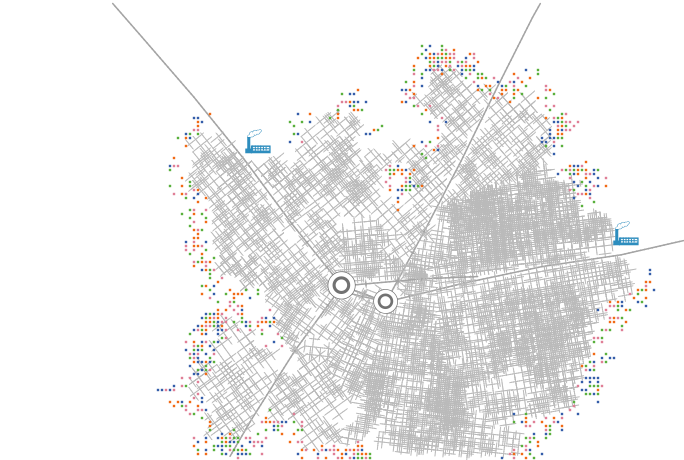
\includegraphics[width=0.33\textwidth]{Figures/Reproducibility/stdView}
\hfill
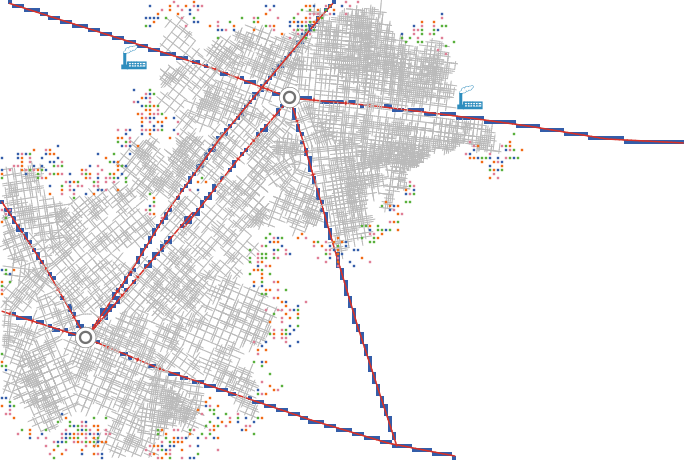
\includegraphics[width=0.33\textwidth]{Figures/Reproducibility/ViewRoads}
\hfill
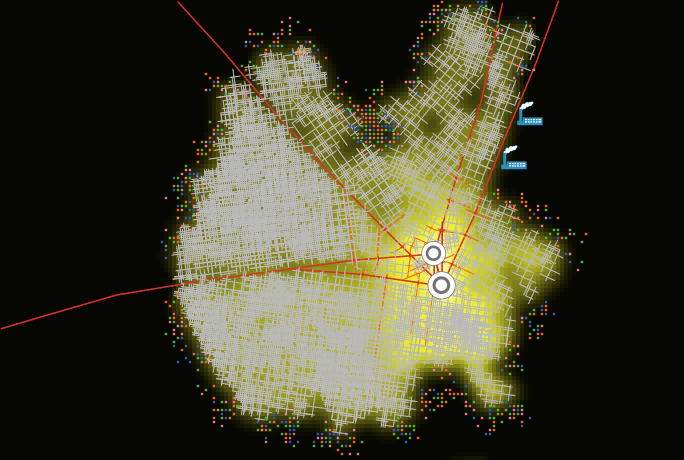
\includegraphics[width=0.33\textwidth]{Figures/Reproducibility/landValues_cityFinished}
\caption[Reproducibility and visualization][Reproductibilité et visualisation]{Example of simple improvement in visualization that can help understanding mechanisms implied in the model. \textit{Left: } Example of original output ; \textit{Middle: } Visualization of main roads (in red) and underlying patches attribution, suggesting possible implementation bias in the use of discretized trace of roads to track their positions ; \textit{Right: }Visualization of land values using a more readable color gradient. This step confirms the hypothesis, through the form of value distribution, that the morphogenesis step is an unnecessary detour to generate a random field for which simple diffusion method should provide similar results, as detailed in the paragraph on implementation.}{Exemple d'amélioration simple dans la visualisation qui peut aider à appréhender les mécanismes impliqués par le modèle. \textit{Gauche : } Exemple de sortie originale ; \textit{Centre : } Visualisation des routes principales (en rouge) et de l'attribution des patches sous-jacente, qui suggère de possibles biais d'implémentation dans l'utilisation de la trace discrete des routes pour garder trace de leur position ; \textit{Droite : } Visualisation des valeurs foncières en utilisant un gradient de couleur plus lisible. Cette étape confirme l'hypothèse, par la forme de la distribution des valeurs, que l'étape de morphogenèse est un détour non-nécessaire pour générer un champ aléatoire pour lequel des simples mécanismes de diffusion devrait fournir des résultats similaires, comme détaillé dans le paragraphe sur l'implémentation. \comment{(Florent) on ne peut pas comprendre ce que tu dis juste en regardant ces trois images. tu dois mieux accompagner le lecteur}}
\label{fig:example_tij_viz}
\end{figure}
%%%%%%%%%%%%%%%%%%%%%



\subsection{On the Need of Exactitude in Model Implementation}{Sur le besoin d'exactitude dans l'implémentation du modèle}

% Barthelemy paper, pb in model description/implementation
%  - test different analyses with possible biaises -


\bpar{
Possible divergences between model description in a paper and the effectively implemented processes may have grave consequences on the final reproducibility. The road network growth model given in~\cite{barthelemy2008modeling} is one example of such a discrepancy. A strict implementation of model mechanisms provide slightly different results than the one presented in the paper, and as source code is not provided we need to test different hypotheses on possible mechanisms added by the programmer (that seems to be a connexion rule to intersections under a certain distance threshold). Lessons that could be possibly drawn from this examples are 
\begin{itemize}
\item the necessity of providing source code
\item the necessity of providing architecture description along with code (if model description is in a langage too far from architectural specifications) in order to identify possible implementation biaises
\item the necessity of performing and detailing explicitly model explorations, that would in that case have helped to identify the implementation bias.
\end{itemize}
}{
Des divergences potentielles entre la description du modèle dans un article et les processus effectivement implémentés peut avoir des conséquences graves sur la reproductibilité finale. Le modèle de croissance du réseau routier donné dans~\cite{barthelemy2008modeling} est un exemple d'une telle discrépance. Une implémentation stricte des mécanismes du modèle produit des résultats légèrement différents de ceux présentés dans le papier, et comme le code source n'est pas fourni nous devons tester différentes hypothèses sur des mécanismes possibles ajoutés par le programmeur (qui semble être une règle de connexion aux intersections sous un certain seuil de distance). Des leçons qui peuvent éventuellement être tirées de cet exemple sont
\comment{(Florent) déjà dit non ?}[pas exactement même façon et pas même contexte]
\begin{itemize}
\item la nécessité de fournir le code source
\item la nécessité de fournir une description de l'architecture en même temps que le code (si la description du modèle est faite dans un langage trop loin de spécification architecturales) afin d'identifier des biais possibles d'implémentation
\item la nécessité de procéder à des explorations explicites du modèle et de les détailler, ce qui dans ce cas aurait permis d'identifier de possibles biais d'implémentation.
\end{itemize}
}



\bpar{
Making the last point mandatory may ensure a limited risk of scientific falsification as it is generally more complicated to fake false exploration results than to effectively explore the model. One could imagine an experiment to test the general behavior of a subset of the scientific community regarding reproducibility, that would consist in the writing of a false modeling paper in the spirit of~\cite{zilsel2015canular}, in which opposite results to the effective results of a given model are provided, without providing model implementation. A first bunch of test would be to test the acceptance of a clearly non-reproducible paper in diverse journals, possibly with a control on textual elements (using or not ``buzz-words'' associated to the journal, etc.). Depending on results, a second experiment may be tested with providing open source code for model implementation but still with false results, to verify if reviewers effectively try to reproduce results when they pretend to want the code (in reasonable computational power limits of course, HPC being not currently broadly available in Humanities).
}{
Rendre le dernier point obligatoire pourrait assurer un risque limité de falsification puisqu'il est généralement plus compliqué de falsifier des résultats d'exploration plutôt que d'explorer effectivement le modèle. \comment{(Florent) joint project.. : on n'a pas à connaitre tes side-projects}
 On pourrait imaginer une expérience pour tester le comportement général d'un sous-ensemble de la communauté scientifique au regard de la reproducibilité, qui consisterait en l'écriture d'un faux papier de modélisation
}


\subsection{Perspectives}{Perspectives}


\bpar{
Again, reproducibility and transparency is a non-negotiable feature of contemporaneous science, along with Open practices and Open Access. Too much examples (see a very recent one in experimental economics~\cite{camerer2016evaluating}) show in various disciplines the lack of reproducibility of experiments, that is a falsification of previous results or a result in itself. Falsification is a costly practice, and even if necessary~\cite{chavalarias2005nobel}, could be made more efficient through more transparency and direct reproducibility, increase therein the global workflow of science. We develop in parallel of this thesis various tools aimed to ease reproducibility, for which an overview is given in appendix~\ref{app:workflow}.
}{

}




\subsection{Interactive Exploration and Production of Results}{Exploration interactive et production des résultats}

L'usage d'applications interactives pour la fouille de données a des avantages non discutables, tel qu'une familiarisation avec la structure des données par une vue d'ensemble qui serait beaucoup plus laborieuse voire impossible autrement. C'est la même idée sous-jacente qui justifie l'interactivité pour l'exploration préliminaire des modèles basé-agent intégrée à des plateformes comme Netlogo~\cite{wilensky1999netlogo} ou Gamma [Cit. gamma]. C'était d'ailleurs un objectif couplé qu'avait initialement~\cite{rey2015plateforme}, c'est à dire une intégration complète de l'exploration fine des modèles et de la production des graphes de sortie ainsi que leur exploration interactive. Comme le rappelle R. Reuillon (Entretien du 11/04/2017, voir \ref{app:data:interview}), la plateforme OpenMole qui devait accueillir cette couche supplémentaire était loin d'être mature à l'époque et ne l'est toujours pas aujourd'hui, puisque l'état de l'art de telles pratiques est en pleine construction et bouleversements réguliers~\cite{holzinger2014knowledge}. Des difficultés au regard de la reproductibilité, qui nous concernent particulièrement ici, sont récurrentes et loin d'être résolues. En effet, il faut bien situer la position de ces outils et méthodes comme une aide cognitive préliminaire\footnote{que nous ne jugeons pas superficielle puisque nous les mobilisons au moins par deux fois par la suite, voir \ref{} et \ref{}}, mais peu souvent comme permettant la production de résultats finaux : lorsque les paramètres ou dimension se multiplient, l'export d'un graphe est bien souvent déconnecté de l'information complète ayant conduit à sa production. De la même manière, l'utilisation de notebooks intégrés tel Jupyter, permettant d'intégrer analyses et rédaction du compte-rendu, peut devenir dangereux car on peut justement revenir sur un script, tester différentes valeurs d'un paramètre, et perdre les valeurs qui avaient produit un graphe donné. L'utilisation de versioning peut être une solution partielle mais souvent lourde. Dans l'idéal, tout logiciel interactif permettant l'export de résultats devrait en même temps exporter un script ou une description exacte et utilisable permettant d'arriver exactement à ce point à partir des données brutes.







